% !TEX program = lualatex
\documentclass[aspectratio=43,professionalfonts,handout]{beamer}
\usepackage{beamer_template}

\newcommand{\LectureNum}{10}
\newcommand{\LectureTitle}{分数関数（１）}
\newcommand{\TextPages}{p.\,91-93}
\newcommand{\NextTopic}{分数関数（２）}
\newcommand{\NextPages}{p.\,93}
\newcommand{\CourseName}{基礎数学B}
\renewcommand{\TermName}{前期}

\begin{document}

% -----------------------------------------------
% スライド1: 表紙＋目標＋用語・定義
% -----------------------------------------------
\begin{frame}{\CourseName\quad 第\LectureNum 回「\LectureTitle 」}
  {\small \TermName\quad \TeacherName\quad ／\quad 教科書 \TextPages\quad
  \textbf{目標}：y=a/x のグラフ（双曲線）と漸近線を理解できる}

  \begin{block}{用語・定義}
  \begin{description}[labelwidth=5.5em]
    \item[\kw{分数関数}] ~
    \item[\kw{双曲線}] ~
    \item[\kw{漸近線}] ~
  \end{description}
  \end{block}
\end{frame}

% -----------------------------------------------
% スライド2: 公式・性質
% -----------------------------------------------
\begin{frame}{公式・性質}
  \begin{block}{}
  \begin{itemize}
    \item y=a/x：定義域・値域・漸近線・象限
    \item y=a/(x-p)+q：漸近線 x=p と y=q
  \end{itemize}
  \end{block}
\end{frame}

% -----------------------------------------------
% スライド3: 図・グラフ（TikZコードを手動追加）
% -----------------------------------------------
\begin{frame}{図・グラフ}
  \centering
  % TODO: y=1/x（基本形）と y=1/(x-1)+2（平行移動）と漸近線
  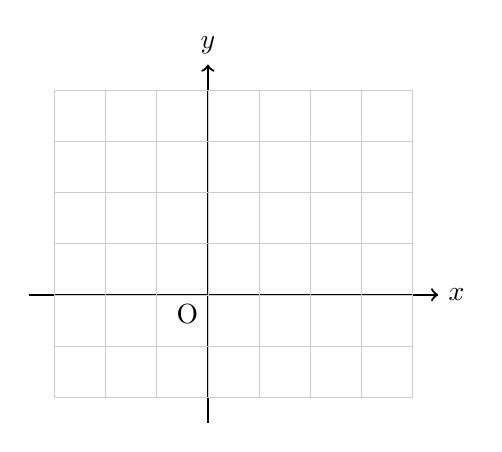
\begin{tikzpicture}[scale=0.65]
    \draw[->,thick] (-3.5,0) -- (4.5,0) node[right]{$x$};
    \draw[->,thick] (0,-2.5) -- (0,4.5) node[above]{$y$};
    \node[below left] at (0,0) {O};
    \draw[gray!40, very thin] (-3,-2) grid (4,4);
    % ここにグラフを描画
  \end{tikzpicture}
\end{frame}

% -----------------------------------------------
% スライド4: 例1→問1
% -----------------------------------------------
\begin{frame}{例1→問1}
  \begin{exampleblock}{例題1) p.92（定義域・値域・漸近線・グラフ）}
    （板書で解説）
  \end{exampleblock}

  \vfill

  \begin{block}{問3) p.92（3問）\quad 自分で解いてみよう}
    （ノートに解くこと）
  \end{block}
\end{frame}

% -----------------------------------------------
% スライド5: 補足演習
% -----------------------------------------------
\begin{frame}{補足演習}
  \begin{block}{練習2-A 問3・問4) p.99\quad 自分で解いてみよう}
    （ノートに解くこと）
  \end{block}
  % NOTE: 例が1セットのみのため補足演習に充てる
\end{frame}

% -----------------------------------------------
% まとめ
% -----------------------------------------------
\begin{frame}{まとめ}
  \begin{itemize}
    \item y=a/x のグラフは双曲線、漸近線は x=0 と y=0
    \item y=a/(x-p)+q は漸近線が x=p と y=q に移動する
    \item 定義域・値域は漸近線の「除外点」から読み取る
  \end{itemize}

  \vfill
  {\small 基本問題：173}
\end{frame}

\end{document}
